\documentclass[letterpaper]{article}
\usepackage[margin=1in]{geometry}
\usepackage[utf8]{inputenc}
\usepackage{textcomp}
\usepackage{amssymb}
\usepackage{natbib}
\usepackage{graphicx}
\usepackage{gensymb}
\usepackage{amsthm, amsmath, mathtools}
\usepackage[dvipsnames]{xcolor}
\usepackage{enumerate}
\usepackage{mdframed}
\usepackage[most]{tcolorbox}
\usepackage{csquotes}
% https://tex.stackexchange.com/questions/13506/how-to-continue-the-framed-text-box-on-multiple-pages

\tcbuselibrary{theorems}

\newcommand{\R}{\mathbb{R}}
\newcommand{\Z}{\mathbb{Z}}
\newcommand{\N}{\mathbb{N}}
\newcommand{\Q}{\mathbb{Q}}
\newcommand{\C}{\mathbb{C}}
\newcommand{\code}[1]{\texttt{#1}}
\newcommand{\mdiamond}{$\diamondsuit$}
\newcommand{\PowerSet}{\mathcal{P}}
\newcommand{\Mod}[1]{\ (\mathrm{mod}\ #1)}
\DeclareMathOperator{\lcm}{lcm}

%\newtheorem*{theorem}{Theorem}
%\newtheorem*{definition}{Definition}
%\newtheorem*{corollary}{Corollary}
%\newtheorem*{lemma}{Lemma}
\newtheorem*{proposition}{Proposition}


\newtcbtheorem[number within=section]{theorem}{Theorem}
{colback=green!5,colframe=green!35!black,fonttitle=\bfseries}{th}

\newtcbtheorem[number within=section]{definition}{Definition}
{colback=blue!5,colframe=blue!35!black,fonttitle=\bfseries}{def}

\newtcbtheorem[number within=section]{corollary}{Corollary}
{colback=yellow!5,colframe=yellow!35!black,fonttitle=\bfseries}{cor}

\newtcbtheorem[number within=section]{lemma}{Lemma}
{colback=red!5,colframe=red!35!black,fonttitle=\bfseries}{lem}

\newtcbtheorem[number within=section]{example}{Example}
{colback=white!5,colframe=white!35!black,fonttitle=\bfseries}{def}

\newtcbtheorem[number within=section]{note}{Important Note}{
        enhanced,
        sharp corners,
        attach boxed title to top left={
            xshift=-1mm,
            yshift=-5mm,
            yshifttext=-1mm
        },
        top=1.5em,
        colback=white,
        colframe=black,
        fonttitle=\bfseries,
        boxed title style={
            sharp corners,
            size=small,
            colback=red!75!black,
            colframe=red!75!black,
        } 
    }{impnote}
\usepackage[utf8]{inputenc}
\usepackage[english]{babel}
\usepackage{fancyhdr}
\usepackage[hidelinks]{hyperref}

\pagestyle{fancy}
\fancyhf{}
\rhead{CSE 101}
\chead{Wednesday, March 9, 2022}
\lhead{Lecture 23}
\rfoot{\thepage}

\setlength{\parindent}{0pt}

\begin{document}

\section{NP-Completeness}
We continue our discussion on NP-Completeness. 

\subsection{Problem: Zero-One Equations}
To prove more complicated reductions, it is helpful to have the correct problem to prove the reductions from. Sometimes, you might need to build intermediate problems that are nice to work with, mainly for convenience. 

\bigskip 

One convenient problem is the \textbf{zero-one equation}. Given a matrix $A$ with only \code{0}'s and \code{1}'s as entries and a vector $b$ of only \code{1}'s, determine whether or not there is an $x$ with \code{0} and \code{1} entries so that 
\[Ax = b\]
The problem is clearly in NP. We will show that is NP-complete. 

\subsubsection{Example: Zero-One Equations}
Find an $x_1, x_2, x_3$ such that 
\[\begin{bmatrix}
    1 & 0 & 1 \\ 1 & 1 & 0
\end{bmatrix} \begin{bmatrix}
    x_1 \\ x_2 \\ x_3
\end{bmatrix} = \begin{bmatrix}
    1 \\ 1
\end{bmatrix}\]
is satisfied. Equivalently, does there exist $x_1, x_2, x_3 \in \{0, 1\}$ such that 
\[\begin{cases}
    x_1 + x_3 = 1 \\ 
    x_1 + x_2 = 1
\end{cases}\]
holds? 

\begin{mdframed}[]
    It's not hard to see that this holds.     
\end{mdframed}

Generally, this is what a zero-one equation looks like; a bunch of sets of $x_i$'s that need to add to \code{1}. 

\subsubsection{Reducing 3-SAT to Zero-One Equation}
The idea behind reducing a 3-SAT formula to a zero-one equation is that we'll look at the formulation of 3-SAT and use one term from each clause. 

\bigskip 

We will create one variable for each term to denote whether or not it has been selected. Then, we'll add equations to enforce exactly one term from each clause such that no contradictory terms are selected. 

\bigskip 

To see this in action, we consider an example. Consider the following 3-SAT instance 
\[(\underbrace{x}_{x_1} \lor \overbrace{y}^{x_2} \lor \underbrace{z}_{x_3}) \land (\overbrace{\overline{x}}^{x_4} \lor \underbrace{y}_{x_5}) \land (\overbrace{\overline{y}}^{x_6} \lor \underbrace{\overline{x}}_{x_7})\]
\begin{itemize}
    \item We can translate this into the following zero-one equation instance by noting that we have one term per clause. That is: 
    \[\begin{cases}
        x_1 + x_2 + x_3 = 1 \\ 
        x_4 + x_5 = 1 \\ 
        x_6 + x_7 = 1
    \end{cases}\]
    \item We now want to make sure we don't select any contradictory terms. For example, we can't select both $x_1$ and $x_4$. So, if we use inequalities, we get something like: 
    \[\begin{cases}
        x_1 + x_4 \leq 1 \\ 
        x_1 + x_7 \leq 1 \\ 
        x_2 + x_6 \leq 1 \\ 
        x_5 + x_6 \leq 1
    \end{cases}\]
    So, if both $x_1$ and $x_4$ are \code{1}, then we have a problem. In any case, if we satisfy this system of inequalities of zero-one variables $x_1$ through $x_7$, then this is equivalent to having a solution to the original 3-SAT problem. 
    \item We note that we do not allow inequalities. A zero-one equation is only allowed to have \emph{equalities}. So, we need to tweak this system to make this equalities instead. An easy trick to do just this is to introduce a new variable. That is, if we had the inequality $a + b \leq 1$, then we can replace it with $a + b + c = 1$. The point is, if $a + b \leq 1$, then this will hold if and only if there is a zero-one variable $c$ such that $a + b + c = 1$. To see what we mean, we note that if $a + b = 0$, then we let $c = 1$; likewise, if $a + b = 1$, then $c = 0$. And, as usual, if $a + b = 2$, then we have an issue either way. 
    
    \bigskip 

    So, we have the system of \emph{equalities}: 
    \[\begin{cases}
        x_1 + x_4 + x_8 = 1 \\ 
        x_1 + x_7 + x_9 = 1 \\ 
        x_2 + x_6 + x_{10} = 1 \\ 
        x_5 + x_6 + x_{11} = 1
    \end{cases}\]
\end{itemize}
In general, the construction is as follows: 
\begin{itemize}
    \item Create one variable per term. 
    \item For each clause, create one equation. 
    \item For each pair of contradictory term, create an equation with those two and a new variable, and set that equal to one. 
\end{itemize}
This gives us a system of zero-one equations, which is satisfiable if and only if the original 3-SAT problem is. 

\subsubsection{Another Way of Looking at Zero-One Equations}
Suppose we treat $A$ as a bunch of column vectors. Recall that if $A = \begin{bmatrix}
    v_1 & v_2 & v_3 & \dots & v_n
\end{bmatrix}$, then we have 
\[Ax = x_1 v_1 + x_2 v_2 + \dots + x_n v_n\]
So, let's suppose we have the following matrix declaration 
\[A = \begin{bmatrix}
    1 & 0 & 1 \\ 0 & 0 & 1 \\ 0 & 1 & 1 \\ 1 & 1 & 0 
\end{bmatrix}\]
and we wanted to solve for $Ax = \vec{1}$. Then, we can write 
\[
    x_1 \begin{bmatrix}
        1 \\ 0 \\ 0 \\ 1
    \end{bmatrix} + x_2 \begin{bmatrix}
        0 \\ 0 \\ 1 \\ 1
    \end{bmatrix} + x_3 \begin{bmatrix}
        1 \\ 1 \\ 1\\ 0
    \end{bmatrix} = \begin{bmatrix}
        1 \\ 1 \\ 1 \\ 1
    \end{bmatrix}
\]
We can rewrite this like so 
\begin{equation*}
    \begin{aligned}
        &x_1 \begin{bmatrix}
            1 & 0 & 0 & 1
        \end{bmatrix} + \\ 
        &x_2 \begin{bmatrix}
            0 & 0 & 1 & 1
        \end{bmatrix} + \\ 
        &x_3 \begin{bmatrix}
            1 & 1 & 1 & 0
        \end{bmatrix} \\ 
        &= \begin{bmatrix}
            1 & 1 & 1 & 1
        \end{bmatrix}
    \end{aligned}
\end{equation*}
This is a bit suggestive because the way this was written implies that you could treat this as an addition of numbers. If we did this addition without performing any carries, this would almost be exactly the same computation as if we were adding numbers rather than adding vectors.

\bigskip 

Let's pretend we actually did addition of numbers. 
\begin{verbatim}
            x1 *    1 0 0 1     +
            x2 *    0 0 1 1     + 
            x3 *    1 1 1 0
            ---------------------
            =       1 1 1 1
\end{verbatim}
We have these three numbers and we want to see if there is some $x_1, x_2, x_3$ such that $x_1$ times the first number plus $x_2$ times the second number plus $x_3$ times the third number is equal to the solution. The only difference between adding numbers and adding vectors is that if we add numbers and we get big-enough terms, we might need to deal with carry-overs. For example, if we were doing base 2 addition, then we will get a carry over if we added 1 with 1. But, if we added these numbers in a high-enough base (e.g. base 10), we can't possibly get big-enough terms that will give us a carry over.

\bigskip 

So, if the numbers are represented in a large enough base (e.g. base 1000) that carrying is impossible, we have a solution to the vector equation if and only if we have a solution to the number equation. 


\subsection{Subset Sum}
What we just talked about actually relates naturally to the subset sum problem. 

\bigskip 

\textbf{Problem Statement:} Given a set $S$ of numbers and a target number $C$, is there a subset $T \subseteq S$ whose elements sum to $C$? 

\bigskip 

\textbf{Alternatively:} Can we find an $x_y \in \{0, 1\}$ such that 
\[\sum_{y \in S} x_y y = C\]
where
\[x_y = \begin{cases}
    0 & \text{If } y \text{ is not in the subset.} \\ 
    1 & \text{If } y \text{ is in the subset.} 
\end{cases}\]
Essentially, we want to find some setting of these binary variables so that the sum of all $y$ in the set of $x_y y$ is equal to the target. 

\subsubsection{Reducing Zero-One Equations to Subset Sum}
The alternative point that we've made can actually be used to relate the problem to zero-one equations. The idea is that we replace all of these vectors with numbers in base $n$ where $n$ is big enough so that there is no carry over with the arithmetic, and since the base is big enough that we'll never have to do any carry over, the vector addition problem is exactly equivalent to the number addition problem here. 

\bigskip 

Asking whether or not there is some zero-one linear combination of these numbers that add up to another number is equivalent to asking if there is a subset of these numbers which add up to the target. 

\bigskip 

So, starting from the instance of a zero-one equation, we can reduce the instance of subset sum with the same answer, which gives us the desired reduction. 

\bigskip 

Therefore, subset sum is NP-complete. 

\subsection{Generalized (Non-Repeated) Knapsack}
Subset sum is pretty closely related to the (non-repeated) knapsack. In particular: 
\begin{itemize}
    \item Subset sum wants to find a set of values so that the weights equal the capacity. 
    \item Knapsack wants to find a set of values so that the weights are at most the capacity and the value is as large as possible. 
\end{itemize}
There's a pretty easy way to get rid of this ``value'' idea. 

\subsubsection{Reducing Subset Sum to Knapsack}
We can reduce subset sum to knapsack in the following way. 
\begin{itemize}
    \item We create a knapsack problem where, for each item, the value of the item is just the weight of the item. Then, this becomes a ``the price is right'' knapsack; you want to find some set of items where the total weight is as large as possible without going over the capacity. 
    \item Maximizing the value is the same as maximizing the weight without going over the capacity. 
    \item We can, then, achieve a certain value (which is the capacity) if and only if there is a subset of the items with toatl weight equal to the capacity. So, if we want to answer the question ``is it possible to find a set of these items where the total weight is equal to the capacity?'' then this is exactly the same as the subset sum problem. 
\end{itemize}
So, this gives us a pretty natural reduction from subset sum to knapsack. Therefore, knapsack is NP-Hard. 

\subsubsection{Relation to Polynomial-Time Runtime Knapsack}
Our dynamic programming algorithm that we discussed some time ago was polynomial time in the \emph{total weight} (in terms of the numerical values of the weights). In this case, this is exponential. 


\subsection{Hamiltonian Cycles}
We want to show that Hamiltonian Cycles (and thus Traveling Salesman Problem) are NP-Complete (and NP-Hard). We will use a reduction from zero-one equations to Hamiltonian Cycles to show this. 

\subsubsection{Strategy}
Very often, to show that some problem is NP-Complete, we want to be able to show that it can simulate that logic somehow. This is difficuly for Hamiltonian Cycles as most graphs have too many options, so we will want to find specific graphs with clear, binary choices. 

\bigskip 

This is difficult for Hamiltonian cycle as most graphs have too many options in terms of the edges, so we want to find specific graphs with clear, binary choices. 

\bigskip 

To see how this would work, let's consider an example. 
\begin{itemize}
    \item First, start with a cycle. 
    \begin{center}
        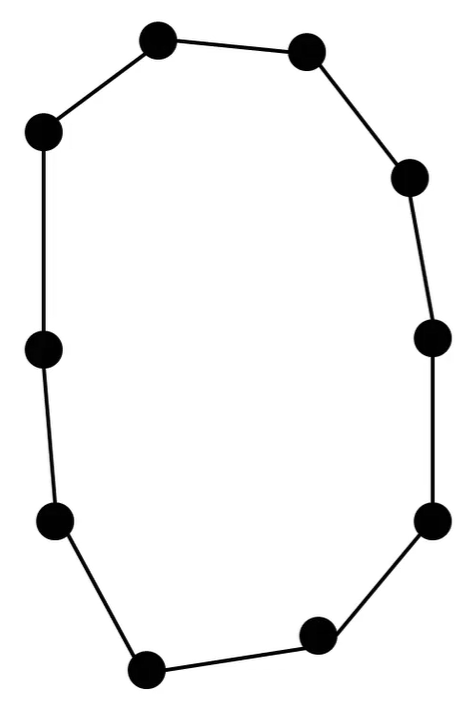
\includegraphics[scale=0.35]{../assets/zoe_ham_1.png}
    \end{center}
    There is clearly a Hamiltonian cycle here.

    \item Then, for some of these edges, we can double them up. That is, rather than 
    \begin{center}
        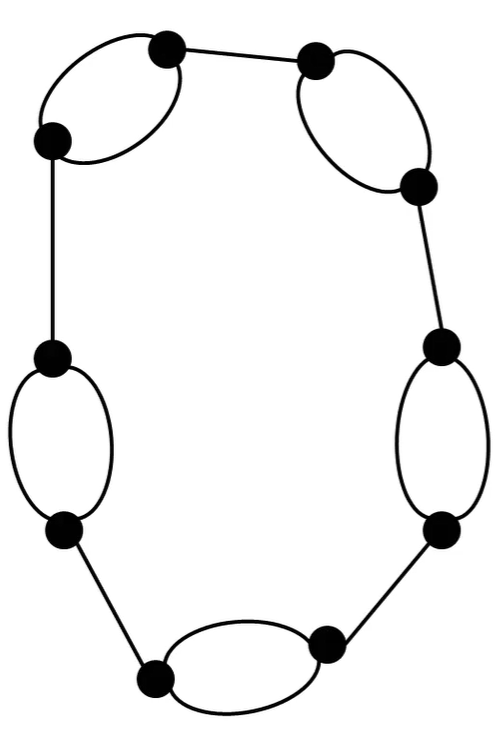
\includegraphics[scale=0.35]{../assets/zoe_ham_2.png}
    \end{center}
    This graph still has a Hamiltonian cycle. But, now, there are multiple ways to find a Hamiltonian cycles (there are many binary choices that can be made here). At the moment, our construction has no constraints on these choices; we can pick whatever combinations of these binary choices we want and still get a Hamiltonian cycle. But, at least, we have a prototype of a graph where trying to find a Hamiltonian cycle on this graph involves making a specific collection of (in this case) binary choices, which is a good place to start if we want to make some NP-Completeness reductions. Now, at least, there is some \emph{logic} involved. We just need to add some limitations as to what choices we can make. 

    \bigskip 

    So, to sumamrize, in our cycle, we must pick one edge from each pair, which provides a nice set of binary variables. 

    \item We need to add restrictions so that we can't just use any collection of choices. We need to make it difficult to figure out whether it is possible to make the right choices or not. To do so, we make use of a \emph{gadget}. 
    \begin{center}
        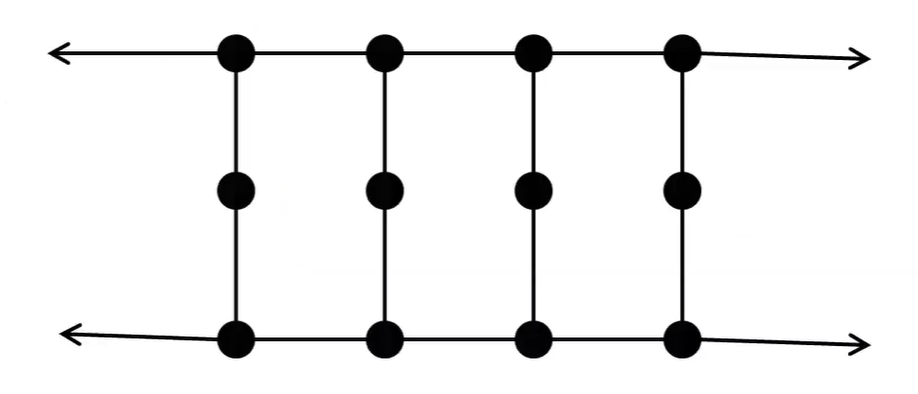
\includegraphics[scale=0.35]{../assets/zoe_ham_3.png}
    \end{center}
    Gadgets are generally useful for proving NP-Completeness/Hardness reduction problems. It's not necessarily well-defined; it's essentially just a piece of construction which only has a few ways it can be filled out. It often allows us to enforce some condition or simulate some more complicated behavior. So, in our case here, this gadget will be a subgraph of the full graph we made. We have a collection of edges and vertices, and there are these four edges with arrows which connects the gadget to the rest of the graph.
    
    \bigskip 

    If this gadget is part of the graph and there is a Hamiltonian cycle in this graph, then we note that, because of these degree 2 vertices, any Hamiltonian cycle has to visit these vertices. The only way it can do that is if it uses both edges on each of the columns (the red edges below).
    \begin{center}
        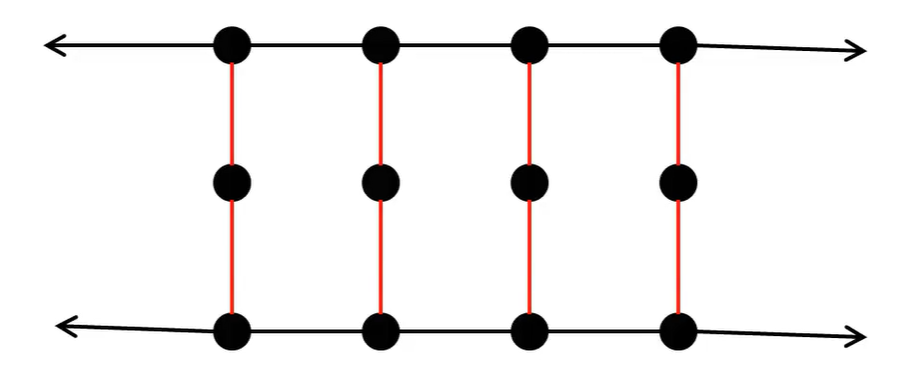
\includegraphics[scale=0.35]{../assets/zoe_ham_4.png}
    \end{center}

    When we get to the top or bottom of one of these columns, the vertex at the top or bottom of the columns has to connect to exactly one of its left or right neighboring vertices. We can't just connect these vertices however we want, or else we might have a disconnected cycle in the middle. 

    \bigskip 

    There are only two ways to fill these edges out and still be consistent with having a Hamiltonian cycle; both of those ways involve a zig-zag pattern (see the two graphs below). 
    \begin{center}
        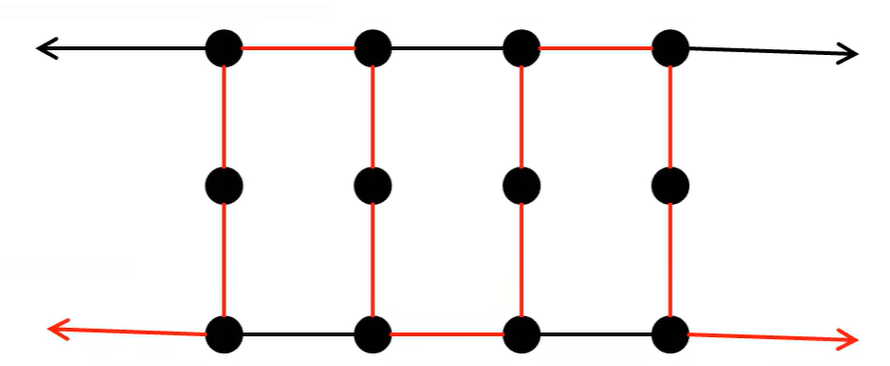
\includegraphics[scale=0.3]{../assets/zoe_ham_5.png}
        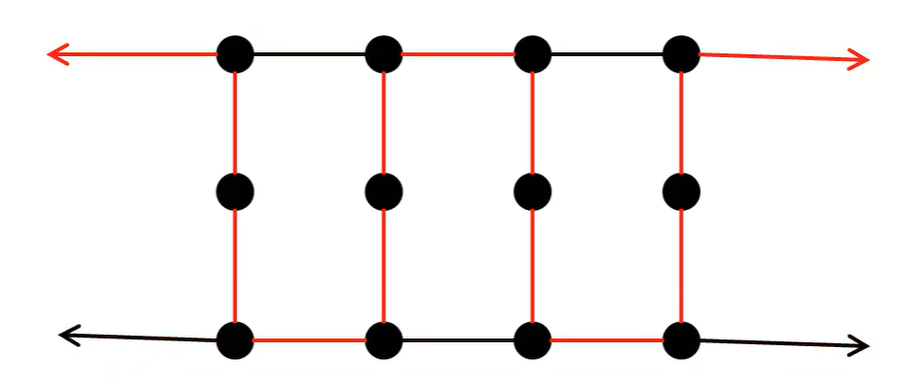
\includegraphics[scale=0.3]{../assets/zoe_ham_6.png}
    \end{center}
    To see how this gadget used, suppose we have a giant cycle, and in the middle of this cycle we have these two binary choices that can be made. 
    \begin{center}
        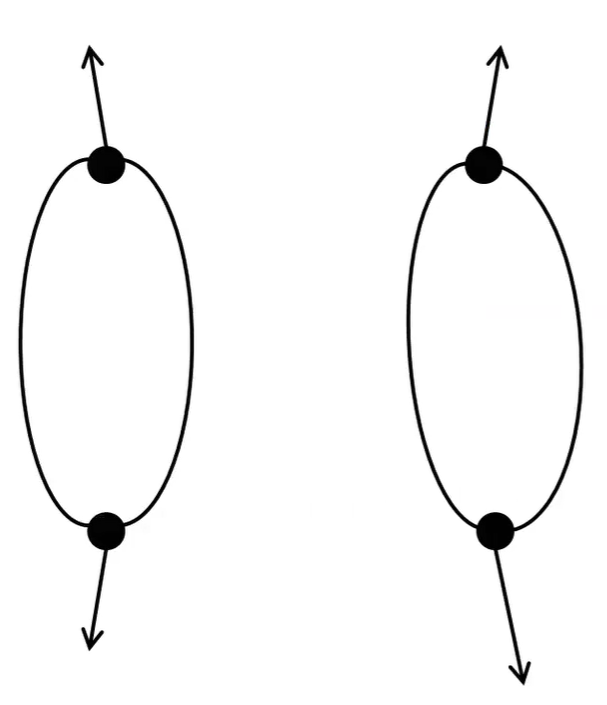
\includegraphics[scale=0.35]{../assets/zoe_ham_7.png}
    \end{center}
    We can then hook the gadget up between these pair of edges. 
    \begin{center}
        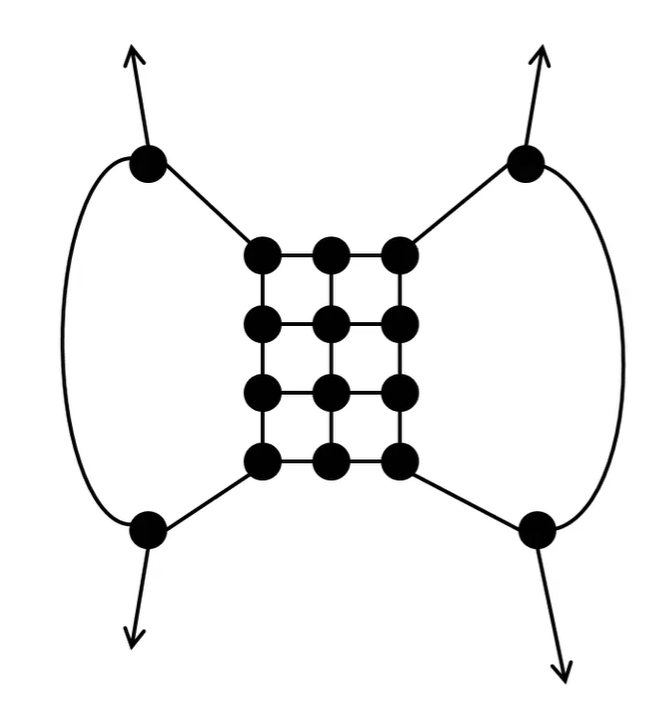
\includegraphics[scale=0.35]{../assets/zoe_ham_8.png}
    \end{center}
    There are two ways to fill out ths gadget.
    \begin{center}
        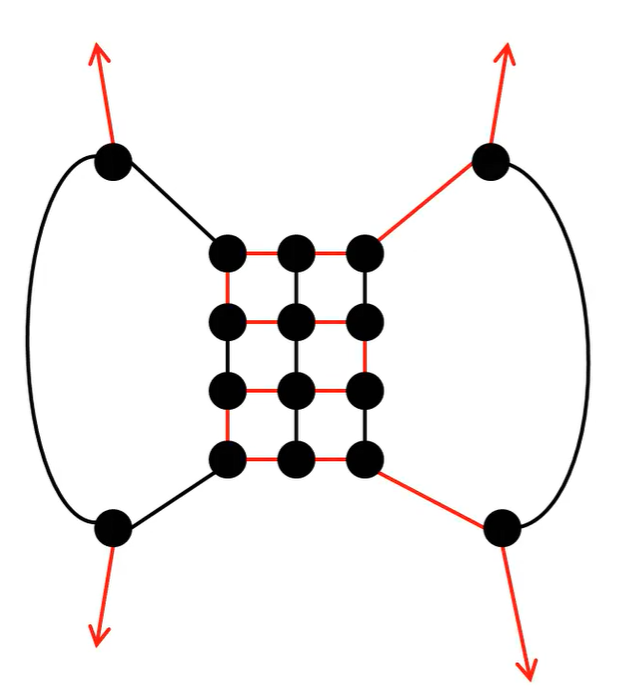
\includegraphics[scale=0.30]{../assets/zoe_ham_9.png}
        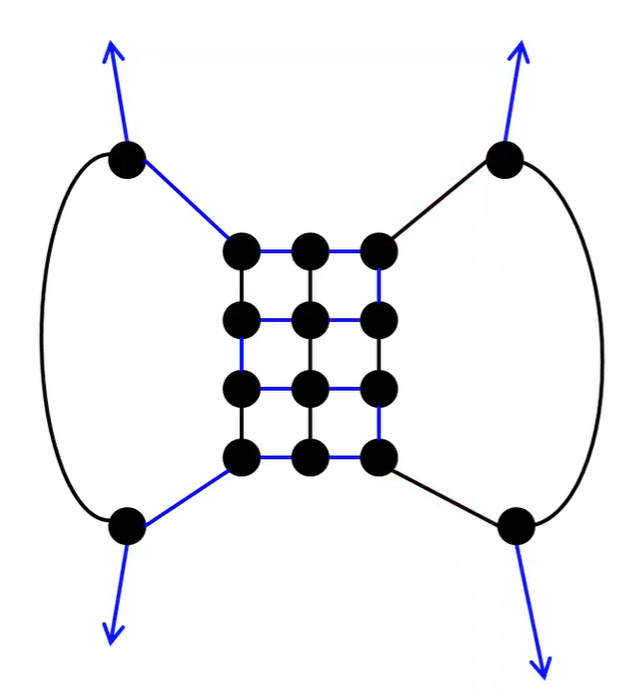
\includegraphics[scale=0.30]{../assets/zoe_ham_10.png}
    \end{center}
    This allows us to force logic upon our choices. By doing this for several pairs of edges, we can construct a Hamiltonian cycle problem equivalent to the following:  
    \begin{itemize}
        \item You are given a number of choices where you need to pick one from several options (of multi-edges). 
        \item You have several constraints that say that of the two choices you could make, you must have picked exactly one of them. 
    \end{itemize}
    With this in mind, we want to see if you can simulate a hard problem from this. 
\end{itemize}
Now, we can talk about the zero-one equation. 
\begin{itemize}
    \item For each variable, choose either 0 or 1. This will tell you the value of that variable.
    \item For each equation, choose one variable to be equal to 1.
    \item We also need to add some constraints. For each variable that appears in an equation, exactly one of the following should be selected. Either that variable is in the equation, or that variable is equal to 0. 
\end{itemize}

\subsubsection{Example: Zero-One Equation}
Suppose you have the following zero-one equation 
\[\begin{cases}
    x_1 + x_2 + x_3 = 1 \\ 
    x_2 + x_4 = 1
\end{cases}\]

First, we can build a graph for each gadget. 
\begin{center}
    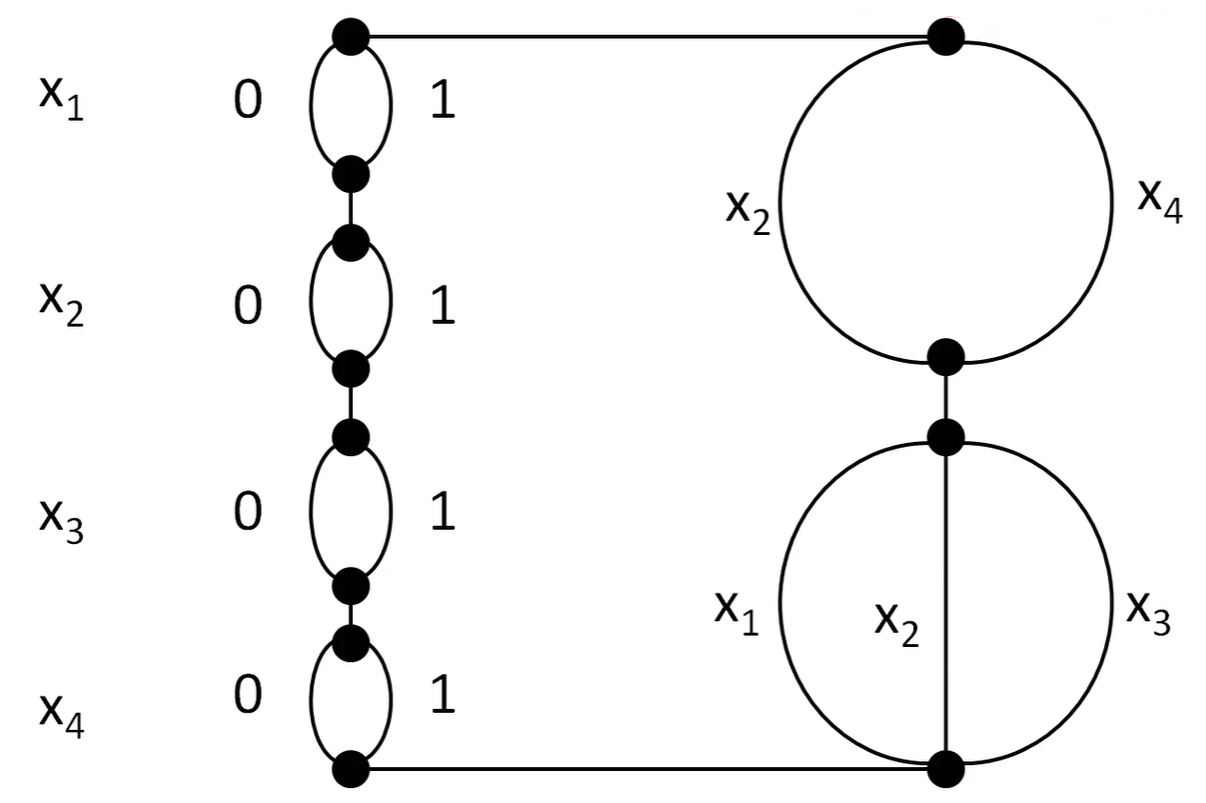
\includegraphics[scale=0.30]{../assets/zoe_ham_12.png}
\end{center} 
For each variable that appears in each equation, we have a gadget which enforces the constraint that we either select a variable or we set that variable equal to 0. 
\begin{center}
    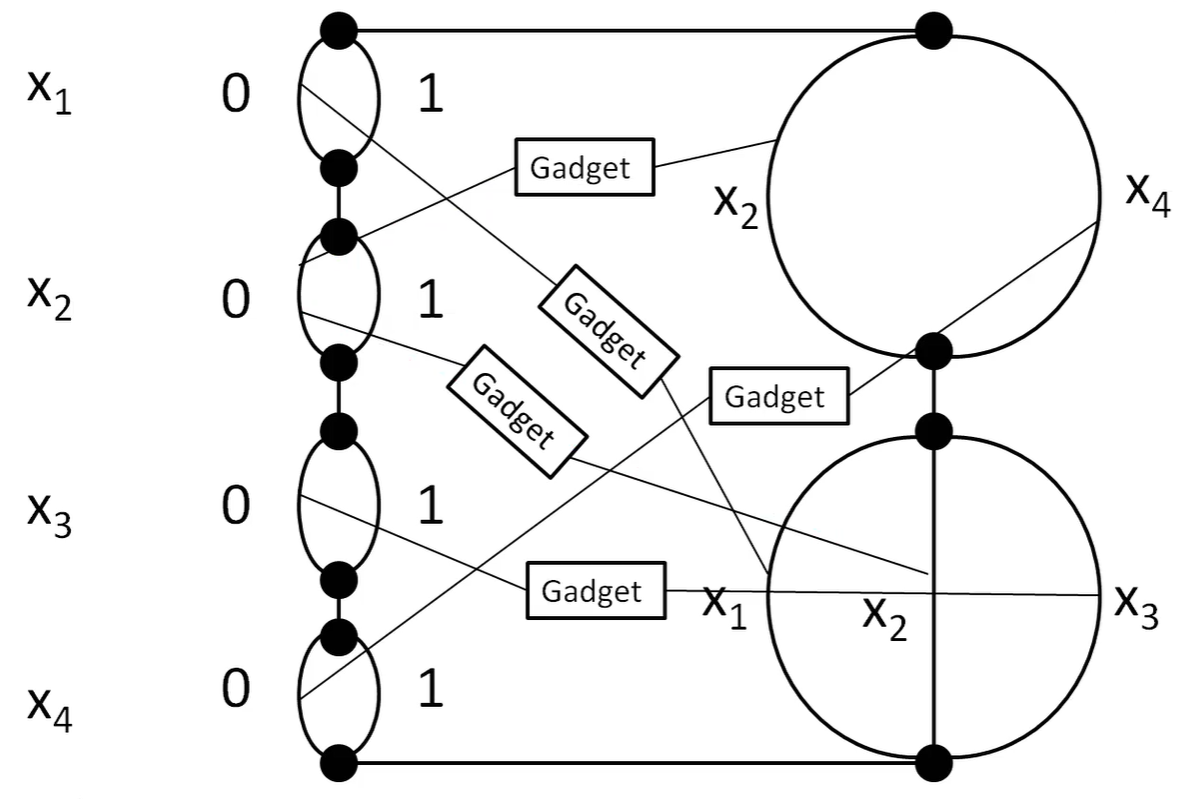
\includegraphics[scale=0.30]{../assets/zoe_ham_11.png}
\end{center} 
To see what this means, consider the top gadget. This is saying that either: 
\begin{itemize}
    \item Either $x_2$ will be selected from the equation. 
    \item Or we set $x_2$ equal to 0. 
\end{itemize}
This gives us a complicated Hamiltonian cycle problem, but this graph that we built has a Hamiltonian cycle if and only if the corresponding zero-one equation has a solution. Consider the following: 
\begin{center}
    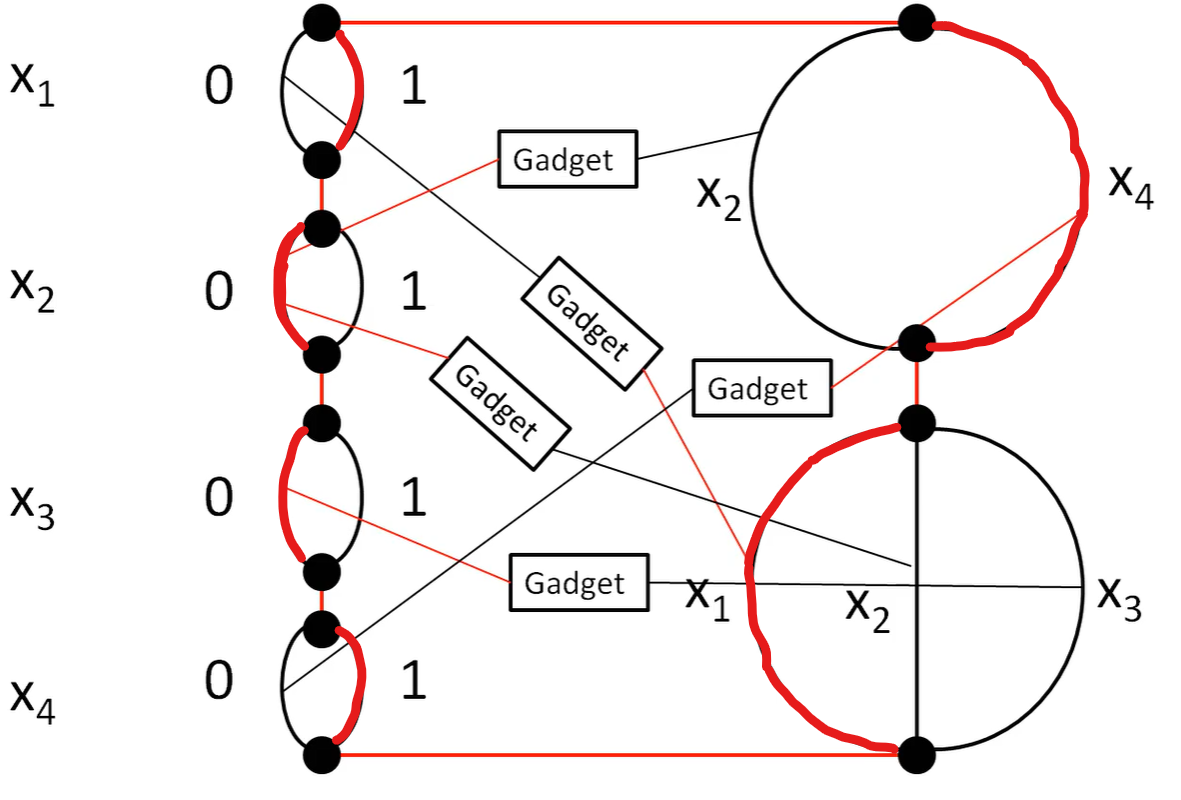
\includegraphics[scale=0.3]{../assets/zoe_ham_13.png}
\end{center}
Here, we are saying that $x_1 = 1$, $x_2 = x_3 = 0$, and $x_4 = 1$. 

\subsection{Reduction Summary}
\begin{center}
    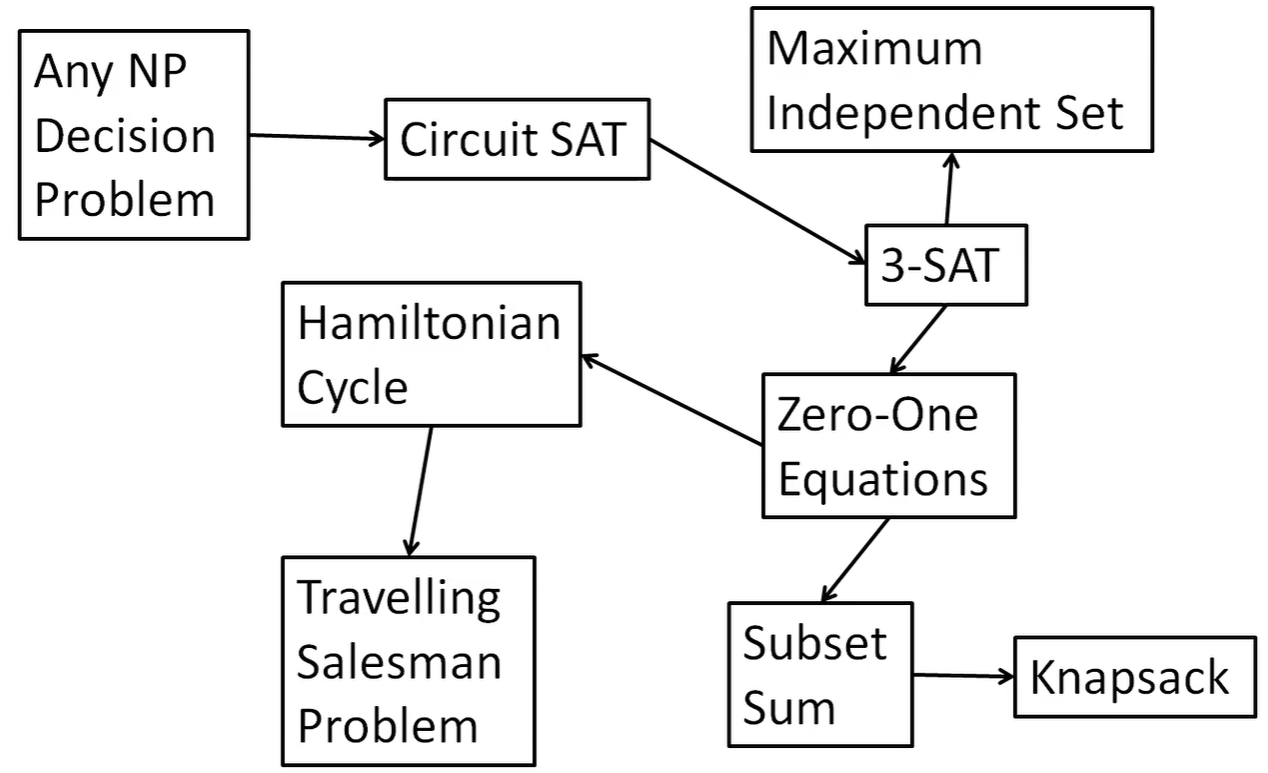
\includegraphics[scale=0.3]{../assets/reduction_summary.png}
\end{center}

\end{document}